% \begin{table}[H]
%   \caption{\centering Average Hourly Earnings \emph{(universe)} \newline Of Production Workers in Manufacturing \emph{(classification)} \newline in the United States \emph{(area)} \newline $1950-1952$ \emph{(time)} }\label{tab:exampleTable}
%   \small
%   \centering
%   \begin{tabular}{lccccr}
%   \toprule[\heavyrulewidth]\toprule[\heavyrulewidth]
%   \textbf{C1} & \textbf{C2} & \textbf{C3} & \textbf{C4}\\ 
%   \midrule
% \multirow{3}{*}{\textbf{Row}}& Val & Val & \textcolor{igreen}{GreenVal}\\
%   & & Val  & \textcolor{igreen}{Val}\\
% & &  & \textcolor{igreen}{Example}\\ \hdashline
%   \bottomrule[\heavyrulewidth] 
%   \end{tabular}
% \end{table}


% Example Algorithm and pseudocode
\begin{algorithm}
\caption{An algorithm with caption}\label{alg:cap}
\begin{algorithmic}
\Require $n \geq 0$
\Ensure $y = x^n$
\State $y \gets 1$
\State $X \gets x$
\State $N \gets n$
\While{$N \neq 0$}
\If{$N$ is even}
    \State $X \gets X \times X$
    \State $N \gets \frac{N}{2}$  \Comment{This is a comment}
\ElsIf{$N$ is odd}
    \State $y \gets y \times X$
    \State $N \gets N - 1$
\EndIf
\EndWhile
\end{algorithmic}
\end{algorithm}




\begin{figure}
    \centering
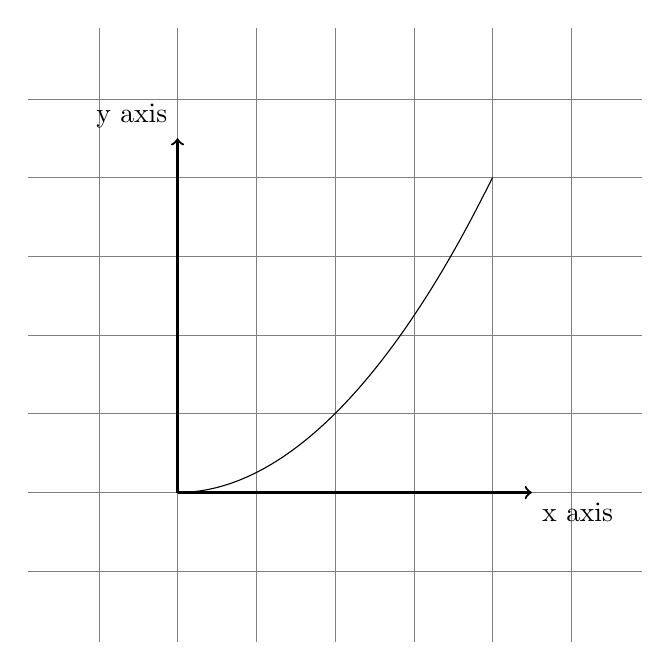
\begin{tikzpicture}
    \draw[step=1cm,gray,very thin] (-1.9,-1.9) grid (5.9,5.9);
    \draw[thick,->] (0,0) -- (4.5,0) node[anchor=north west] {x axis};
    \draw[thick,->] (0,0) -- (0,4.5) node[anchor=south east] {y axis};
    \draw (0,0) parabola (4,4);
\end{tikzpicture}
\caption{Example TikZ Figure}
\end{figure}